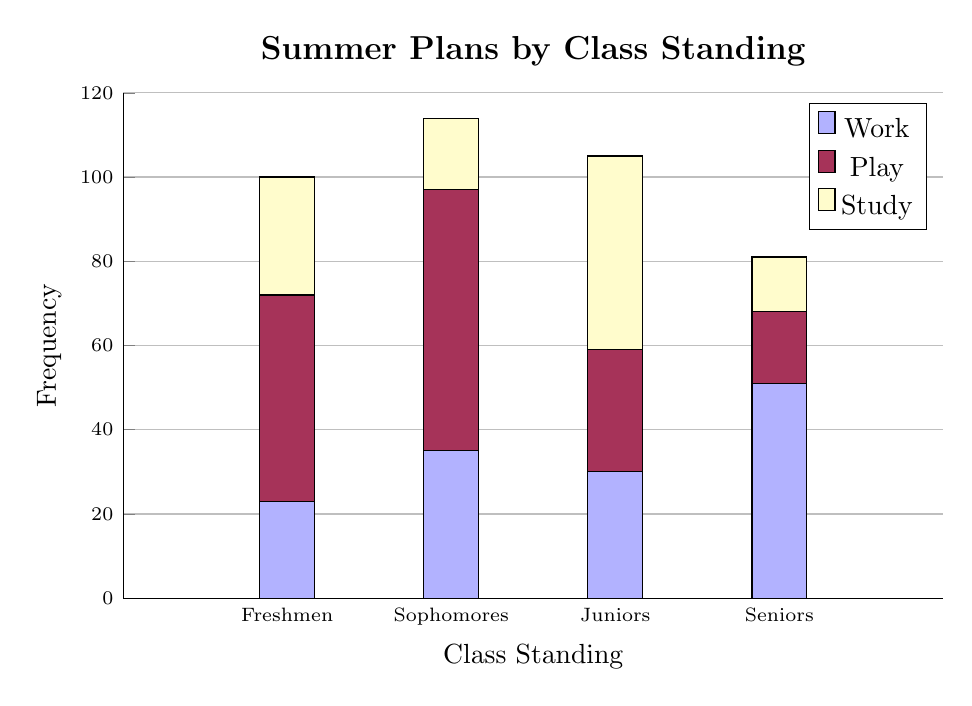
\begin{tikzpicture}[
    declare function={binom(\k,\n,\p)=\n!/(\k!*(\n-\k)!)*\p^\k*(1-\p)^(\n-\k);}
  ]
  \begin{axis}[
      axis lines*=left,
      no markers,
      xmin = 0, xmax=15, ymin=0, ymax=120,
      xtick={3,6,9,12},
      ytick={0,20,...,120}, 
      xticklabels={Freshmen,Sophomores,Juniors,Seniors},
      ticklabel style={font=\scriptsize},
      xlabel={Class Standing},
      ylabel={Frequency},
      title={\large\bf Summer Plans by Class Standing},
      enlargelimits=false,
      clip=false,
      grid = none,
      ymajorgrids=true,
      ybar stacked,
      bar width=1,
      width=12cm,
      height=8cm
    ]
    \addplot+[draw=black,fill=blue!30] coordinates { 
        (3,23) (6,35) (9,30) (12,51)
    };
    \addplot+[draw=black,fill=purple!60!gray] coordinates { 
        (3,49) (6,62) (9,29) (12,17)
    };
    \addplot+[draw=black,fill=yellow!20!white] coordinates { 
        (3,28) (6,17) (9,46) (12,13)
    };
    \legend{\strut Work, \strut Play, \strut Study}
  \end{axis}
\end{tikzpicture}
